\documentclass{ieeeaccess}
\usepackage{cite}
\usepackage{amsmath,amssymb,amsfonts}
\usepackage{algorithmic}
\usepackage{graphicx}
\usepackage{textcomp}
\usepackage[locale = DE]{siunitx}
\usepackage[colorlinks=true]{hyperref}
\usepackage[capitalise]{cleveref}
\usepackage[justification=centering,small,sc]{caption}
\usepackage{csquotes}
\usepackage{enumitem}
\usepackage{float}

\graphicspath{{./}}

% Legendas em português (o template define TABLE/FIGURE)
\renewcommand{\tablename}{Tabela}
\renewcommand{\figurename}{Figura}

\def\BibTeX{{\rm B\kern-.05em{\sc i\kern-.025em b}\kern-.08em
    T\kern-.1667em\lower.7ex\hbox{E}\kern-.125emX}}
\begin{document}
\history{Especialização em Computação Científica para a Indústria}
\doi{Trabalho de Conclusão de Curso. Turma 2024}
\dataDaDefesa{10{\slash}09{\slash}2025}
\title{Estudo de Caso de uma Arquitetura Modular para Previsão de Readmissão em UTI com MIMIC-IV}
\author{
    \uppercase{Renan de Almeida Simões Braga}\authorrefmark{1}
    \uppercase{Pedro Giassi}\authorrefmark{1}
}
\address[1]{Instituto Federal de Educação, Ciência e
Tecnologia de Santa Catarina, Florianópolis, SC 88020-300 Brasil (e-mail: renan.asb1989@aluno.ifsc.edu.br, pedro.giassi@ifsc.edu.br)}

\markboth{Especialização de Computação Científica para a Indústria. 2023-2}{}

\begin{abstract}
A readmissão não planejada em unidade de terapia intensiva (UTI) associa-se a maior mortalidade e custo assistencial, e a decisão de alta ainda se apoia essencialmente no julgamento clínico. Este trabalho propõe e avalia uma arquitetura modular de apoio à decisão para previsão de readmissão em UTI dentro de 72 horas, aplicada à base MIMIC-IV v3.1. A arquitetura adapta ao contexto intra-UTI a estratégia de \textit{snapshots} temporais originalmente concebida para o pronto-socorro: quatro classificadores independentes são treinados sobre janelas cumulativas de 24 horas (D0 a D3), cada um utilizando apenas as variáveis disponíveis até o respectivo corte. Sobre uma coorte de 65.760 estadias de 48.524 pacientes, com taxa de readmissão de 4,5\%, compararam-se quatro algoritmos e um \textit{ensemble}, com hiperparâmetros otimizados por Optuna e divisão em nível de paciente. Uma auditoria do conjunto de variáveis removeu o tempo total de permanência --- conhecido apenas na alta e, portanto, indisponível no instante da predição --- e uma variável redundante, ao custo de 0,002 de AUC. O melhor modelo resultante (XGBoost em D2) alcançou AUC-ROC de 0,644, com sensibilidade de 0,62 e precisão de 0,083 no ponto de operação adotado. A interpretação por SHAP indica predominância da carga crônica de comorbidade sobre o estado fisiológico agudo e mostra que a importância das variáveis muda entre os cortes temporais, o que sustenta a arquitetura por \textit{snapshots}. A ponderação de classes usada contra o desbalanceamento, porém, compromete a calibração das probabilidades e restringe seu uso agregado. Discute-se por que esse patamar é compatível com a literatura metodologicamente rigorosa e por que valores próximos a 0,80 relatados para o mesmo problema decorrem sobretudo de populações específicas e de reamostragem sintética anterior à validação.
\end{abstract}


\begin{keywords}
Aprendizado de Máquina, Calibração de Modelos, Explicabilidade de Modelos, MIMIC-IV, Readmissão em UTI, Sistema de Apoio à Decisão Clínica, XGBoost
\end{keywords}


\titlepgskip=-15pt

\maketitle

% ---------------------------------------------------------
% 1. Introdução
% ---------------------------------------------------------
\section{Introdução}
\subsection*{A. Justificativa}
A Unidade de Terapia Intensiva (UTI) representa um dos ambientes mais complexos e dinâmicos da medicina moderna. Profissionais de saúde lidam com um volume massivo de dados fisiológicos, gerados em tempo real, onde decisões rápidas e precisas são cruciais. A digitalização desses registros --- cuja adoção nos hospitais norte-americanos saltou de 9\% para 96\% desde 2008 --- tornou esse volume acessível a métodos computacionais \cite{Patton2023}. A dificuldade não reside apenas no volume, mas na própria natureza imprevisível da condição humana em estado crítico. \cite{Gardner2014}, em sua análise sobre sistemas de monitoramento em UTI, destacam essa complexidade e a lacuna tecnológica existente:

% --- CITAÇÃO DIRETA EM INGLÊS ---
\begin{displayquote}
\small
\textit{We are able to record and process physiologic signals with much greater capability than we did just a decade ago, but we are still failing to collect those data in a timely manner, how to generate alerts and assist care-givers to provide optimum patient care. [...] Not only is the human body complex with its multiple internal control systems, each individual is genetically different, and each of these control systems have been injured or damaged [...] Thus, we may have a few hundreds of models of commercial airplane crashes but we have billions of models of human pathology.}\footnote{Tradução nossa: Somos capazes de registrar e processar sinais fisiológicos com uma capacidade muito maior do que há uma década, mas ainda estamos falhando em coletar esses dados de maneira oportuna, em como gerar alertas e auxiliar os cuidadores a fornecer o cuidado ideal ao paciente. [...] Não apenas o corpo humano é complexo com seus múltiplos sistemas de controle interno, como cada indivíduo é geneticamente diferente, e cada um desses sistemas de controle foi lesionado ou danificado [...] Assim, podemos ter algumas centenas de modelos de acidentes de aviões comerciais, mas temos bilhões de modelos de patologia humana.}
\end{displayquote}
% ------------------------------------

\noindent % Remove a indentação do parágrafo seguinte
Esta passagem evidencia o desafio central: a capacidade humana, por si só, é insuficiente para processar a "bilhões de modelos de patologia" em tempo hábil para a tomada de decisão. É precisamente nesta lacuna que a inteligência artificial (IA) se torna imprescindível. Um sistema de apoio à decisão, como o proposto neste trabalho, pode analisar esses dados complexos, identificar padrões de risco de readmissão que seriam imperceptíveis a um observador humano e, assim, fornecer o suporte necessário para otimizar o cuidado e a gestão de recursos na UTI --- desde que superadas as barreiras que separam um modelo validado de um sistema em uso clínico \cite{Kelly2019}.

Entre as decisões tomadas nesse ambiente, a alta da UTI é das mais consequentes e das menos instrumentadas. A readmissão não planejada associa-se a mais que o dobro do risco de mortalidade, além de maior tempo de internação e maior consumo de recursos \cite{Koumantakis2025}. Diferentemente de um erro de prescrição ou de um diagnóstico tardio, ela decorre de um julgamento de prontidão para o qual existem escores propostos --- NEWS, MEWS e o índice de estabilidade e carga de trabalho para transferência --- mas nenhum de uso rotineiro consolidado \cite{Badilla2025}: na prática, o clínico decide a partir da sua leitura do paciente.


\subsection*{B. Definição do Problema}
O problema tem duas faces, e a literatura recente permite delimitar as duas com precisão.

A primeira é de engenharia. Apesar da profusão de modelos de aprendizado de máquina em ambiente acadêmico, poucos chegam à prática clínica por falta de arquiteturas que cubram o ciclo completo: ingestão, processamento, treinamento, validação, implantação, monitoramento e \textit{feedback}. Um classificador com bom desempenho em um \textit{notebook} não é um sistema; falta-lhe a definição reprodutível da coorte, a serialização consistente entre treino e inferência, a explicação da predição e a previsão de como será mantido quando os dados mudarem --- lacunas reconhecidas tanto na literatura de engenharia de sistemas de aprendizado de máquina \cite{Sculley2015} quanto na de translação clínica de IA \cite{Kelly2019}.

A segunda é metodológica, e é menos discutida. A revisão sistemática mais abrangente sobre readmissão em UTI reuniu 24 estudos e 49 modelos e encontrou heterogeneidade praticamente total entre os desempenhos publicados --- $I^2 = 99{,}96\%$ ---, com apenas dois dos 24 estudos submetidos a validação externa; em um deles, a área sob a curva ROC caiu de 0,80 para 0,55 fora da base de origem \cite{Koumantakis2025}. Levantamento independente identificou vazamento de dados afetando ao menos 294 artigos em 17 disciplinas \cite{Kapoor2023}. A consequência prática é que não existe, hoje, um valor de referência confiável para o problema: um trabalho novo não tem contra o que se comparar, e um desempenho aparentemente modesto pode ser simplesmente o desempenho honesto.

É nessa interseção que este trabalho se posiciona --- uma arquitetura que cubra o ciclo completo e, ao mesmo tempo, produza um resultado auditável, em que cada decisão metodológica capaz de inflar a métrica seja explicitada e, quando possível, quantificada.

\subsection*{C. Objetivo Geral}
Propor e avaliar uma arquitetura modular de apoio à decisão clínica para previsão de readmissão em UTI sobre a base MIMIC-IV, adaptando ao contexto intra-UTI a estratégia de \textit{snapshots} temporais de King et al. \cite{King2022}.

O trabalho de referência prevê admissões hospitalares a partir do pronto-socorro de um hospital universitário britânico. Sua contribuição central não é o algoritmo, mas o desenho temporal: em vez de um classificador único, um conjunto de modelos XGBoost é aplicado em instantes sucessivos desde a chegada do paciente, cada um treinado apenas com o que já havia sido registrado até aquele ponto da visita. Sobre 109.465 visitas, obtiveram-se valores de AUROC entre 0,82 e 0,90 conforme o tempo decorrido, e as probabilidades individuais foram agregadas para estimar o número de admissões esperado em janelas futuras, com erro médio de 4,0 admissões contra 6,5 do método de referência do hospital \cite{King2022}.

A transposição proposta aqui preserva o desenho e troca os três elementos que definem o problema: a visita ao pronto-socorro passa a ser a internação na UTI, os instantes medidos em minutos passam a blocos cumulativos de 24 horas, e o desfecho de admissão passa a ser a readmissão em até 72 horas após a alta da UTI. Como prova de conceito, implementa-se o pipeline completo, da ingestão do banco à interface de inferência com explicação individual da predição.

\subsection*{D. Objetivos Específicos}
\begin{enumerate}[label=\arabic*.]
\item Definir uma coorte elegível e um desfecho clinicamente defensáveis, com critérios de exclusão explícitos, e extrair do MIMIC-IV o conjunto de variáveis disponível em cada corte temporal --- demografia, sinais vitais, exames laboratoriais, intervenções e escores de gravidade.
\item Implementar os \textit{snapshots} cumulativos D0 a D3 e treinar modelos independentes por corte, comparando quatro algoritmos e um \textit{ensemble}.
\item Formular variáveis de trajetória que expressem a \textit{direção} da evolução clínica entre cortes, e não apenas o acúmulo de valores extremos desde a admissão.
\item Quantificar o efeito de decisões metodológicas capazes de enviesar a avaliação --- particionamento em nível de paciente, tratamento do desbalanceamento e escolha da janela de agregação --- sobre o desempenho medido.
\item Avaliar os modelos quanto à discriminação (AUROC, AUPRC), à calibração (\textit{Brier score}) e ao comportamento em um ponto de operação clinicamente relevante.
\item Interpretar o modelo final por atribuição SHAP, verificando se os padrões aprendidos são fisiologicamente plausíveis e como variam entre os cortes temporais.
\item Disponibilizar uma interface de inferência que apresente, junto do risco estimado, a decomposição individual da predição.
\end{enumerate}

% ---------------------------------------------------------
% 2. Fundamentação Teórica
% ---------------------------------------------------------
\section{Fundamentação Teórica}

\subsection*{A. Aprendizado de Máquina Aplicado à Saúde}
A adoção de prontuários eletrônicos nos hospitais norte-americanos passou de 9\% para 96\% desde 2008, tornando disponível um volume de dados clínicos estruturados que viabilizou a proliferação de modelos preditivos em terapia intensiva \cite{Patton2023}. Algoritmos supervisionados como XGBoost \cite{Chen2016}, \textit{Random Forest} \cite{Breiman2001} e regressão logística tornaram-se o instrumental padrão para classificação binária de risco sobre esses dados.

A avaliação desses modelos apoia-se em três dimensões distintas, frequentemente confundidas. A \textit{discriminação} --- capacidade de ordenar pacientes por risco --- é medida pela área sob a curva ROC e, em desfechos raros, pela área sob a curva precisão--sensibilidade, que é sensível à prevalência e, por isso, mais informativa quando o evento é infrequente \cite{Saito2015}. A \textit{calibração} --- correspondência entre a probabilidade emitida e a frequência observada --- é medida pelo \textit{Brier score} e por curvas de calibração; um modelo pode discriminar bem e ainda assim produzir probabilidades inutilizáveis em termos absolutos, falha descrita como o calcanhar de Aquiles da análise preditiva \cite{VanCalster2019}. O \textit{ponto de operação} traduz a probabilidade em decisão por meio de um limiar, e é nele que sensibilidade e precisão adquirem significado clínico.

Cabe registrar um achado recorrente da literatura de cuidados críticos: apesar das inovações metodológicas, sistemas de escore desenvolvidos há duas décadas são apenas modestamente superados por métodos modernos de aprendizado de máquina, e a implementação clínica de sistemas preditivos prospectivos permanece um desafio em aberto \cite{Patton2023}. O ganho marginal dos métodos complexos sobre modelos simples, quando ambos operam sobre as mesmas variáveis, é um resultado esperado neste domínio --- e não uma anomalia de um experimento em particular.

\subsection*{B. Readmissão em UTI}
A readmissão à UTI é um fenômeno multifatorial. Revisão sistemática de 28 estudos identifica como fatores mais frequentemente associados a idade, a gravidade da doença, a carga de comorbidades, o tempo de permanência na UTI, o uso de ventilação mecânica e a alta em período noturno \cite{Badilla2025}. Seu impacto é substancial: pacientes readmitidos apresentam mais que o dobro do risco de mortalidade, além de maior tempo de internação e maior consumo de recursos \cite{Koumantakis2025}.

A comparação entre trabalhos da área é dificultada por três fontes de variação raramente explicitadas. A primeira é a definição do desfecho: a janela considerada varia entre 48 horas, 72 horas e 30 dias, e o retorno pode ser contabilizado dentro da mesma internação hospitalar ou em qualquer momento posterior. A segunda é a população: coortes restritas a uma condição específica apresentam taxas de readmissão substancialmente mais altas que as de UTI geral --- 9,6\% e 10,6\% em pacientes com hemorragia intracerebral \cite{Miao2024}, contra valores em torno de 4\% a 5\% em coortes não restritas --- e, por consequência, desempenhos preditivos mais altos. A terceira é o protocolo de avaliação, discutido na seção de resultados. Modelos rigorosos e multicêntricos como o iREAD, validado externamente em duas bases independentes \cite{Lim2025}, são a exceção que evidencia a regra.

\subsection*{C. A Base de Dados MIMIC-IV}
O MIMIC-IV reúne registros desidentificados de internações de um centro médico terciário norte-americano, abrangendo dados demográficos, sinais vitais, exames laboratoriais, prescrições, procedimentos e notas clínicas \cite{Johnson2023}. A base é distribuída pela plataforma PhysioNet \cite{Goldberger2000}, com acesso condicionado a credenciamento e a treinamento em pesquisa com seres humanos, e desidentificação segundo os critérios da legislação norte-americana de privacidade em saúde.

Três características sustentam seu uso como base de referência. A primeira é a publicação da descrição dos dados em periódico revisado por pares \cite{Johnson2023}, o que submete a construção da base ao mesmo escrutínio de um artigo científico. A segunda é o versionamento explícito das entregas, que torna um experimento reproduzível desde que a versão seja declarada --- neste trabalho, a v3.1. A terceira, e a mais relevante do ponto de vista metodológico, é o módulo \texttt{derived}: um conjunto de definições de conceitos clínicos --- escores de gravidade, estágios de lesão renal, janelas de ventilação --- implementadas em consultas públicas e revisadas pela comunidade. Usá-las, em vez de reimplementar cada conceito localmente, elimina uma fonte silenciosa de divergência entre estudos. Deste módulo provêm, neste trabalho, os escores OASIS e de comorbidade de Charlson e o SOFA em janela móvel.

A principal limitação é a contrapartida dessa profundidade: trata-se de um único centro, em um único país, com protocolos assistenciais e perfil populacional próprios --- ao contrário de bases multicêntricas como o eICU-CRD \cite{Pollard2018}. Desempenho obtido sobre o MIMIC-IV não se transfere automaticamente para outro contexto, como discutido nas limitações.

\subsection*{D. Arquiteturas de Apoio à Decisão e Práticas de MLOps}
Sistemas de aprendizado de máquina em produção acumulam custos de manutenção que não são visíveis no código do modelo: o classificador ocupa uma fração pequena de um sistema real, cercada por infraestrutura de coleta, verificação de dados, extração de variáveis, gerenciamento de configuração, monitoramento e servimento \cite{Sculley2015}. Essa assimetria --- muito código em torno de pouco modelo --- é a razão pela qual um classificador com bom desempenho experimental não constitui, por si, um sistema de apoio à decisão, e está entre os obstáculos apontados para a translação de modelos de IA à prática clínica \cite{Kelly2019}.

O conjunto de práticas que endereça essa lacuna consolidou-se sob a denominação MLOps, cujos princípios centrais incluem automação do fluxo, versionamento de dados, código e modelos, reprodutibilidade dos experimentos, monitoramento contínuo em produção e colaboração explícita entre os papéis envolvidos \cite{Kreuzberger2023}. A arquitetura proposta neste trabalho adota o subconjunto mínimo aplicável a uma prova de conceito: modularidade entre etapas, persistência de artefatos que acompanham o modelo --- codificadores, padronizador e a lista ordenada de variáveis --- e definição declarativa e auditável da coorte.

\subsection*{E. \textit{Model Drift} e Recalibração Contínua}
Modelos clínicos degradam com o tempo por dois mecanismos distintos. No \textit{data drift}, a distribuição das variáveis de entrada muda sem que a relação entre elas e o desfecho se altere --- é o caso de uma mudança no perfil etário dos pacientes atendidos. No \textit{concept drift}, é a própria relação entre variáveis e desfecho que muda: um novo protocolo de alta, uma alteração de critério de admissão ou um evento epidemiológico modificam o processo que gera os dados, e o modelo passa a responder a uma pergunta que não é mais a mesma \cite{Finlayson2021}.

O trabalho de referência desta arquitetura oferece um exemplo documentado do segundo caso: seus modelos foram desenvolvidos antes da pandemia de covid-19 e precisaram ser retreinados sobre os dados do período pandêmico, com reavaliação do desempenho sob as novas condições operacionais \cite{King2022}. A resposta usual combina três mecanismos: monitoramento contínuo de discriminação e calibração \cite{VanCalster2019}, recalibração periódica dos componentes mais sensíveis sobre janela móvel recente, e retreinamento completo quando se detecta mudança estrutural \cite{Finlayson2021}. A viabilidade dessas respostas depende diretamente da modularidade da arquitetura --- recalibrar exige que a etapa de calibração seja um componente isolável, e não uma linha de código no meio do treinamento.

\subsection*{F. \textit{Snapshots} Temporais de Paciente}
Um classificador único aplicado a uma internação enfrenta um dilema de enquadramento temporal. Se for treinado sobre variáveis agregadas de toda a internação, utilizará informação que não estava disponível no momento em que a decisão precisa ser tomada --- uma forma de vazamento temporal que infla o desempenho aparente sem qualquer utilidade prospectiva \cite{Kapoor2023}. Se for restrito às primeiras horas, descartará toda a evolução posterior do paciente.

A estratégia de \textit{snapshots} dissolve o dilema ao substituir o classificador único por um conjunto de modelos, um por ponto de decisão, cada qual treinado exclusivamente com o que já havia sido registrado até aquele instante \cite{King2022}. A formulação tem três consequências. A primeira é que cada modelo é honesto por construção quanto à informação disponível. A segunda é que o conjunto permite observar como a importância das variáveis se desloca ao longo do tempo de internação, o que um modelo único não expõe. A terceira é um custo: cortes mais tardios só contêm os pacientes que permaneceram internados até ali, população progressivamente mais selecionada --- de modo que comparar desempenho entre cortes exige cautela, pois as coortes não são as mesmas.

\subsection*{G. Integração de Dados Clínicos (HL7/FHIR) \textit{versus} MIMIC-IV}
Em ambiente hospitalar real, eventos clínicos não chegam como arquivos: são transmitidos como mensagens HL7 v2 ou recursos FHIR --- padrão que reformula a troca de informações clínicas em torno de recursos granulares expostos por interfaces RESTful \cite{Bender2013} ---, roteados por motores de integração e depositados em tabelas de estágio antes de qualquer uso analítico. No Brasil, a adoção de padrões de interoperabilidade para o registro eletrônico em saúde foi regulamentada pelo Ministério da Saúde ainda em 2011, contemplando HL7, CDA, openEHR, ISO 13606-2, TISS e DICOM, além das terminologias SNOMED-CT, LOINC e CID-10 \cite{Araujo2014}. A Rede Nacional de Dados em Saúde, plataforma de integração do Conecte SUS, consolidou esse movimento adotando o HL7 FHIR R4 como padrão de modelagem e troca de informações, com perfis nacionais próprios publicados em guia de implementação \cite{RNDS2024}.

Neste trabalho, esse fluxo é simulado: os arquivos do MIMIC-IV são ingeridos em um banco relacional PostgreSQL e transformados em tabelas analíticas antes de alimentarem o \textit{pipeline}. A equivalência não é completa --- falta o caráter incremental e assíncrono da mensageria real \cite{Bender2013} ---, mas preserva a propriedade que importa para a arquitetura: a camada de ingestão é o único ponto que precisaria ser reescrito para uma implantação sobre FHIR, e as camadas seguintes permanecem inalteradas.


% ---------------------------------------------------------
% 3. Desenvolvimento
% ---------------------------------------------------------
\section{Desenvolvimento}

\subsection*{A. Visão Geral da Arquitetura}
A arquitetura é organizada em cinco camadas, cada uma implementada como um módulo independente que consome e produz artefatos persistidos. Essa separação é deliberada: permite reexecutar qualquer etapa isoladamente e, sobretudo, garante que o artefato usado na inferência seja exatamente o produzido no treinamento --- reprodutibilidade e versionamento são princípios centrais das práticas de MLOps \cite{Kreuzberger2023}.

\begin{enumerate}[label=\arabic*.]
\item \textbf{Ingestão}: carga dos arquivos do MIMIC-IV v3.1 \cite{Johnson2023} em uma instância PostgreSQL, preservando os esquemas originais (\texttt{mimiciv\_hosp}, \texttt{mimiciv\_icu} e \texttt{mimiciv\_derived}).
\item \textbf{Definição da coorte e rotulagem}: consulta SQL única que aplica os critérios de elegibilidade e atribui o desfecho a cada estadia.
\item \textbf{Construção dos \textit{snapshots}}: extração e agregação das variáveis clínicas em quatro cortes temporais cumulativos, com cálculo das variações entre cortes consecutivos.
\item \textbf{Treinamento e seleção}: otimização de hiperparâmetros, validação cruzada, avaliação em conjunto de teste isolado e serialização do modelo junto de seus codificadores.
\item \textbf{Entrega}: interface de inferência que carrega os modelos serializados e devolve, além do risco, a explicação individual da predição.
\end{enumerate}

% [TODO: o arquivo pipeline_readmissao.png ainda não existe — bloco comentado
% para o documento compilar. Reativar quando o diagrama for criado.]
%\begin{figure}[H]
%\centering
%\includegraphics[width=0.95\linewidth]{pipeline_readmissao.png}
%\caption{Pipeline proposto para previsão de readmissão em UTI.}
%\label{fig:pipeline}
%\end{figure}

A arquitetura de referência \cite{King2022} prevê ainda três etapas operacionais posteriores à predição individual: ajuste por curva de sobrevivência, agregação das probabilidades em número esperado de eventos por janela e projeção dos pacientes que ainda se tornarão elegíveis. Este trabalho implementa as cinco camadas descritas acima e discute, na subseção de resultados dedicada à calibração, por que a etapa de agregação exige um passo adicional não contemplado nesta prova de conceito.

\subsection*{B. Definição da Coorte e do Desfecho}
Considera-se readmissão a nova entrada em UTI ocorrida dentro da \textit{mesma internação hospitalar}, com início posterior à alta da UTI índice e dentro de 72 horas. Exige-se intervalo mínimo de quatro horas entre a alta e a nova entrada: retornos imediatos correspondem a movimentações administrativas entre unidades, não a falha na decisão de alta. Janelas curtas são a escolha usual na literatura recente de readmissão precoce --- 48 horas no modelo multicêntrico iREAD \cite{Lim2025}, por exemplo.

A janela de 72 horas foi escolhida por ser clinicamente defensável. A readmissão nesse período reflete, na maioria dos casos, instabilidade já presente no momento da decisão de alta --- ou seja, uma falha no julgamento de prontidão. Após 72 horas passam a dominar fatores independentes do episódio original, como infecções adquiridas na enfermaria, quedas ou procedimentos eletivos, que desvinculam o evento da qualidade daquela decisão. A concentração do risco nas primeiras horas após a saída da UTI é consistente com os fatores identificados na literatura de readmissão precoce \cite{Badilla2025}.

\begin{table}[!t]
\caption{Critérios de elegibilidade da coorte}
\label{tab:criterios}
\centering
\small
\begin{tabular}{p{2.6cm}p{5.0cm}}
\hline
\textbf{Critério} & \textbf{Justificativa} \\
\hline
Idade $\geq$ 18 anos & População adulta \\
Permanência na UTI $\geq$ 4 h & Estadias muito curtas não acumulam observações suficientes \\
Sobrevivência à UTI & Sem alta não há desfecho possível \\
Sem óbito na enfermaria em $\leq$ 72 h sem readmissão & Óbito pós-alta não é readmissão; incluí-lo distorce o denominador \\
Sem transferência para outro hospital & O desfecho deixa de ser observável \\
Sem alta para cuidados paliativos & A readmissão não é o objetivo terapêutico \\
\hline
\end{tabular}
\end{table}

Note-se que não se aplicou o filtro de primeira estadia por paciente: todas as estadias elegíveis entram na coorte, e o risco de vazamento decorrente dessa escolha é tratado na divisão treino/teste descrita na subseção~E.

\subsection*{C. Construção dos \textit{Snapshots} Temporais}
Cada corte $D_n$ agrega os registros desde a admissão na UTI até $(n+1)\times 24$ horas e inclui apenas as estadias com permanência de ao menos esse tempo. A agregação é cumulativa e não deslizante: D2, por exemplo, enxerga tudo o que ocorreu entre a admissão e a hora 72. O desenho segue a formulação por pontos de decisão sucessivos da arquitetura de referência \cite{King2022}.

A estatística de agregação foi escolhida por variável segundo o sentido clínico do extremo, e não de forma uniforme --- critério herdado dos escores de gravidade, que operam sobre o pior valor de cada componente no período \cite{Vincent1996}. Para grandezas em que o valor alto indica gravidade --- creatinina, bilirrubina, ureia, leucócitos --- registra-se o máximo; para aquelas em que a gravidade está no valor baixo --- plaquetas, saturação de oxigênio, pressão sistólica, escala de coma de Glasgow --- registra-se o mínimo; a média acompanha todas, por representar a condição típica do período.

\begin{table}[!t]
\caption{Composição do conjunto de variáveis}
\label{tab:features}
\centering
\small
\begin{tabular}{lr}
\hline
\textbf{Família} & \textbf{Variáveis} \\
\hline
Demografia e contexto da internação & 5 \\
Sinais vitais (12 parâmetros) & 18 \\
Exames laboratoriais (13 exames) & 24 \\
Débito urinário e vasopressores & 6 \\
SOFA calculado (total e 6 componentes) & 7 \\
Estado em janela móvel de 24 h & 14 \\
Escores consolidados (OASIS, Charlson) & 2 \\
\hline
\textit{Extraídas do banco} & \textit{76} \\
Derivadas por engenharia de variáveis & $+12$ \\
Componentes do SOFA removidos & $-6$ \\
\hline
\textbf{Disponíveis ao modelo em D0} & \textbf{82} \\
Variações entre cortes (D1--D3) & $+31$ \\
\hline
\end{tabular}
\end{table}

O escore SOFA é calculado localmente a partir dos seis componentes, aplicando os pontos de corte originais \cite{Vincent1996} a plaquetas, bilirrubina, creatinina, escala de coma de Glasgow \cite{Teasdale1974}, pressão arterial média com suporte vasopressor e relação PaO$_2$/FiO$_2$. Os escores consolidados OASIS \cite{JohnsonOASIS2013} e índice de comorbidade de Charlson \cite{Charlson1987} provêm do módulo \texttt{derived} da própria base. Os seis componentes são removidos do conjunto de treinamento por serem colineares com o total: mantê-los fragmentaria a atribuição de importância entre variáveis redundantes sem acrescentar informação.

Pelo mesmo critério, e por um segundo critério mais estrito, três variáveis foram excluídas após auditoria do conjunto. O tempo total de permanência na UTI, embora presente na tabela de coorte, é medido da admissão até a alta: no corte de 24 horas, conhecê-lo equivale a conhecer o futuro, e seu uso violaria a premissa que sustenta toda a arquitetura de \textit{snapshots}. A variável binária de permanência prolongada, derivada dela, sai junto. A unidade de internação na alta, por sua vez, é idêntica à unidade de admissão em 100\% das estadias --- o MIMIC-IV registra transferências entre unidades de terapia intensiva como estadias distintas ---, de modo que sua presença apenas fragmentava a atribuição de importância entre duas colunas iguais. O efeito dessas remoções sobre o desempenho é quantificado na seção de resultados.

Doze variáveis são derivadas das demais para codificar limiares clinicamente reconhecidos que um modelo de árvore precisaria aprender por partição: índice de choque (frequência cardíaca sobre pressão sistólica), hipotensão grave, taquicardia, relação PaO$_2$/FiO$_2$ e insuficiência respiratória --- esta demarcada em 200, valor que corresponde à síndrome do desconforto respiratório agudo moderada na definição de Berlim \cite{Berlin2012} ---, três faixas de creatinina inspiradas nos estágios de lesão renal aguda \cite{KDIGO2012}, rebaixamento grave e moderado do nível de consciência segundo os cortes usuais da escala de Glasgow \cite{Teasdale1974}, e dois cortes de idade. Registre-se que os estágios de lesão renal aqui empregados usam o valor absoluto de creatinina, e não a razão em relação ao valor basal prevista na diretriz, por indisponibilidade da creatinina prévia à internação.

\subsection*{D. Trajetória Clínica entre Cortes}
Registrar o estado do paciente em cada corte não basta: o que distingue um paciente estável de um em deterioração é a \textit{variação} entre cortes --- e a gravidade no momento da alta é dos fatores mais consistentemente associados à readmissão \cite{Badilla2025}. Calcular essa variação sobre os \textit{snapshots} cumulativos, porém, não funciona --- e esse é um resultado metodológico deste trabalho. Como as agregações cumulativas usam máximo ou mínimo desde a admissão, a diferença entre dois cortes consecutivos é, por construção, sempre não negativa para máximos e sempre não positiva para mínimos. O modelo nunca observa recuperação clínica: um paciente estável e um paciente em melhora produzem exatamente a mesma variação nula.

A solução adotada utiliza a tabela \texttt{sofa} do esquema \texttt{mimiciv\_derived} \cite{Johnson2023}, cujo campo \texttt{sofa\_24hours} aplica a definição original do escore \cite{Vincent1996} sobre uma janela \textit{móvel} de 24 horas a cada hora da internação. Extraindo, para cada corte, o registro mais recente disponível até o limite do corte, obtém-se o estado pontual do paciente naquele instante; a diferença entre dois cortes consecutivos passa então a expressar trajetória real, com sinal negativo indicando melhora. Além do SOFA e de seus componentes, são extraídos em janela móvel a escala de Glasgow, creatinina, plaquetas, bilirrubina, pressão arterial média, débito urinário e relação PaO$_2$/FiO$_2$.

As variações são computadas em dois grupos, com semânticas distintas: sobre as variáveis em janela móvel, capturando trajetória; e sobre as variáveis cumulativas, onde a diferença não indica direção clínica, mas a ocorrência de um novo extremo no período mais recente.

\subsection*{E. Protocolo de Treinamento e Validação}
A divisão treino/teste é feita em nível de paciente, na proporção 80/20: o conjunto de identificadores de paciente é particionado com estratificação pelo desfecho, e todas as estadias de um mesmo indivíduo acompanham seu identificador. Como a coorte inclui múltiplas estadias por paciente, a divisão aleatória por estadia permitiria que o modelo fosse testado em um paciente que já viu no treinamento --- fonte de vazamento cujo efeito é quantificado na comparação entre as versões v1 e v2 dos resultados e cuja prevalência na literatura científica é documentada \cite{Kapoor2023}. A validação cruzada de cinco \textit{folds} usada na busca de hiperparâmetros obedece ao mesmo particionamento.

Os codificadores de variáveis categóricas são ajustados exclusivamente sobre o conjunto de treinamento de cada partição. Categorias não vistas recebem valor sentinela na aplicação, e não provocam reajuste do codificador. Valores ausentes são preenchidos com zero após a substituição de infinitos, sem imputação por média ou por modelo --- decisão conservadora, que evita introduzir informação do conjunto de teste na etapa de preparação, um dos modos de vazamento mais frequentes na literatura revisada \cite{Kapoor2023}. A padronização por escore-z é aplicada apenas à regressão logística; os modelos de árvore operam sobre as variáveis na escala original.

Foram avaliados quatro algoritmos --- regressão logística, \textit{Random Forest} \cite{Breiman2001}, XGBoost \cite{Chen2016} e LightGBM \cite{Ke2017} --- e o \textit{ensemble} por média simples das probabilidades dos dois últimos. A otimização de hiperparâmetros usa Optuna \cite{Akiba2019} com amostrador baseado em estimadores de Parzen estruturados em árvore \cite{Bergstra2011} em modo multivariado, que modela correlações entre parâmetros em vez de tratá-los independentemente, com 50 avaliações por algoritmo em cada corte e a área sob a curva ROC média da validação cruzada como objetivo.

O tratamento do desbalanceamento merece nota. Em vez de fixar o peso da classe positiva na razão entre negativos e positivos --- prática usual ---, o parâmetro entrou no espaço de busca como multiplicador dessa razão. Nenhum reamostramento sintético foi empregado, nem antes nem depois da divisão --- decisão fundamentada na magnitude do viés que a reamostragem anterior à validação introduz \cite{Demircioglu2024}. O limiar de decisão não é 0,5: para cada modelo, escolhe-se na curva precisão--sensibilidade o ponto de maior precisão sujeito à sensibilidade mínima de 0,60, privilegiando a captura do paciente que retornará.

\subsection*{F. Camada de Entrega e Explicabilidade}
Cada corte produz um artefato serializado contendo o modelo treinado, os codificadores, o padronizador, a lista ordenada de variáveis e as métricas obtidas. A lista de variáveis é o que garante que a inferência reproduza exatamente a ordem e o conjunto usados no treinamento, eliminando a divergência entre treino e servimento apontada como fonte recorrente de dívida técnica em sistemas de aprendizado de máquina \cite{Sculley2015}.

A camada de entrega é uma interface interativa em Streamlit que opera em dois modos: consulta por identificador de estadia, recuperando os cortes disponíveis do paciente, e carregamento de arquivo com os dados de um paciente novo. Para cada corte disponível são apresentados o risco estimado, sua evolução ao longo dos cortes e a decomposição da predição por valores SHAP \cite{Lundberg2017}, calculados sob demanda pelo algoritmo TreeSHAP \cite{Lundberg2020}, que obtém atribuições exatas em tempo polinomial para modelos baseados em árvores.

\subsection*{G. Monitoramento e Mitigação de \textit{Drift}}
Modelos clínicos degradam quando a distribuição dos dados ou o processo assistencial mudam --- novos protocolos, mudança no perfil de pacientes, eventos epidemiológicos. O trabalho de referência \cite{King2022} atravessou a pandemia de covid-19 e precisou retreinar seus modelos, e relata desempenho recuperado após o retreinamento; a literatura clínica trata o fenômeno como risco operacional a ser monitorado, e não como eventualidade \cite{Finlayson2021}.

A arquitetura modular proposta contempla essa necessidade por construção: como cada camada persiste seus artefatos, o retreinamento de um corte não exige reexecutar a ingestão nem a construção da coorte --- automação e monitoramento contínuo são justamente os princípios que as práticas de MLOps formalizam \cite{Kreuzberger2023}. O monitoramento previsto acompanha a área sob a curva ROC, o \textit{Brier score} e o erro na contagem agregada de eventos por janela, com recalibração periódica em janela móvel e retreinamento completo quando houver mudança estrutural. Registra-se, contudo, que a operação contínua não faz parte desta prova de conceito: os mecanismos descritos são provisões da arquitetura, não componentes implementados e avaliados.

\subsection*{H. Justificativas Tecnológicas}
PostgreSQL foi adotado por aproximar o ambiente de um cenário hospitalar real, em que os dados clínicos residem em bancos relacionais, e por permitir que a coorte seja definida declarativamente em uma única consulta auditável. XGBoost \cite{Chen2016} e LightGBM \cite{Ke2017} são o padrão de fato para dados tabulares clínicos, com desempenho competitivo e custo computacional compatível com retreinamento frequente. A regressão logística permanece no conjunto avaliado deliberadamente, como linha de base: em problemas clínicos com sinal predominantemente linear, a diferença para os métodos de \textit{boosting} costuma ser pequena \cite{Patton2023}, e reportá-la é uma salvaguarda contra atribuir a um modelo complexo um ganho que ele não produz. Optuna substitui a busca em grade por amostragem adaptativa, viável dentro do orçamento computacional de 400 avaliações. SHAP foi escolhido por fornecer atribuições localmente exatas e aditivas, requisito para que a explicação individual apresentada ao clínico seja reprodutível, e não uma aproximação heurística. Streamlit atende ao propósito de prototipagem da camada de entrega; uma implantação real exigiria uma interface de serviço com autenticação, registro de auditoria e integração via HL7 ou FHIR \cite{Bender2013}.


% ---------------------------------------------------------
% 4. Apresentação dos Resultados
% ---------------------------------------------------------
\section{Apresentação dos Resultados}

\subsection*{A. Coorte e Protocolo de Avaliação}
A aplicação dos critérios de elegibilidade da Tabela~\ref{tab:criterios} ao MIMIC-IV v3.1 \cite{Johnson2023} produziu as coortes da Tabela~\ref{tab:coorte}. Como cada corte exige permanência mínima correspondente na UTI, a população encolhe e se torna progressivamente mais selecionada, e a divisão treino/teste segue o particionamento em nível de paciente descrito na subseção III-E.

\begin{table}[!t]
\caption{Coorte por corte temporal e divisão treino/teste}
\label{tab:coorte}
\centering
\small
\begin{tabular}{lrrrrr}
\hline
\textbf{Corte} & \textbf{Estadias} & \textbf{Pacientes} & \textbf{Readm.} & \textbf{Taxa} & \textbf{Teste} \\
\hline
D0 (0--24 h) & 65.760 & 48.524 & 2.946 & 4,48\% & 13.006 \\
D1 (0--48 h) & 39.516 & 30.831 & 1.933 & 4,89\% & 7.850 \\
D2 (0--72 h) & 25.801 & 20.982 & 1.393 & 5,40\% & 5.195 \\
D3 (0--96 h) & 18.080 & 15.142 & 1.016 & 5,62\% & 3.636 \\
\hline
\end{tabular}
\end{table}

A taxa de readmissão sobe de 4,48\% em D0 para 5,62\% em D3: quem permanece mais tempo na UTI é, de fato, mais grave. O mesmo mecanismo, porém, impede a leitura direta da variação de desempenho entre cortes --- D3 contém apenas os sobreviventes de 96 horas de UTI, população já selecionada e mais homogênea que a de D0.

\subsection*{B. Desempenho Preditivo}
A busca de hiperparâmetros produziu, antes mesmo das métricas, um achado que vale registrar: nos oito ajustes realizados sobre \texttt{scale\_pos\_weight}, o valor ótimo ficou sempre abaixo do desbalanceamento bruto da coorte, entre 41\% e 72\% dele. Compensar integralmente o desbalanceamento, prática comum na literatura, prejudica a ordenação de risco.

\begin{table}[!t]
\caption{AUC-ROC no conjunto de teste, por modelo e corte temporal}
\label{tab:auc}
\centering
\small
\begin{tabular}{lcccc}
\hline
\textbf{Modelo} & \textbf{D0} & \textbf{D1} & \textbf{D2} & \textbf{D3} \\
\hline
Regressão logística & 0,638 & 0,632 & 0,629 & 0,611 \\
Random Forest       & 0,628 & 0,630 & 0,621 & 0,613 \\
XGBoost             & 0,641 & 0,641 & \textbf{0,644} & 0,617 \\
LightGBM            & \textbf{0,642} & 0,641 & 0,639 & 0,618 \\
Ensemble (XGB+LGB)  & \textbf{0,642} & \textbf{0,642} & 0,642 & \textbf{0,619} \\
\hline
\end{tabular}
\end{table}

O melhor resultado global é o XGBoost em D2 (AUC 0,644), seguido do LightGBM e do \textit{ensemble} em D0 (0,642). A diferença entre os quatro algoritmos é pequena --- a regressão logística fica a menos de 0,01 do melhor modelo em D0 ---, o que indica que o sinal disponível é majoritariamente linear e que o ganho de métodos de \textit{boosting} sobre um modelo simples é marginal nesta tarefa, em linha com o que se observa de forma recorrente em predição de desfechos em terapia intensiva \cite{Patton2023}. D3 permanece o corte mais fraco em todos os modelos, resultado da combinação entre coorte menor (14.444 amostras de treino) e população mais homogênea --- restam apenas os pacientes que sobreviveram a 96 horas de UTI.

\begin{figure*}[!t]
\centering
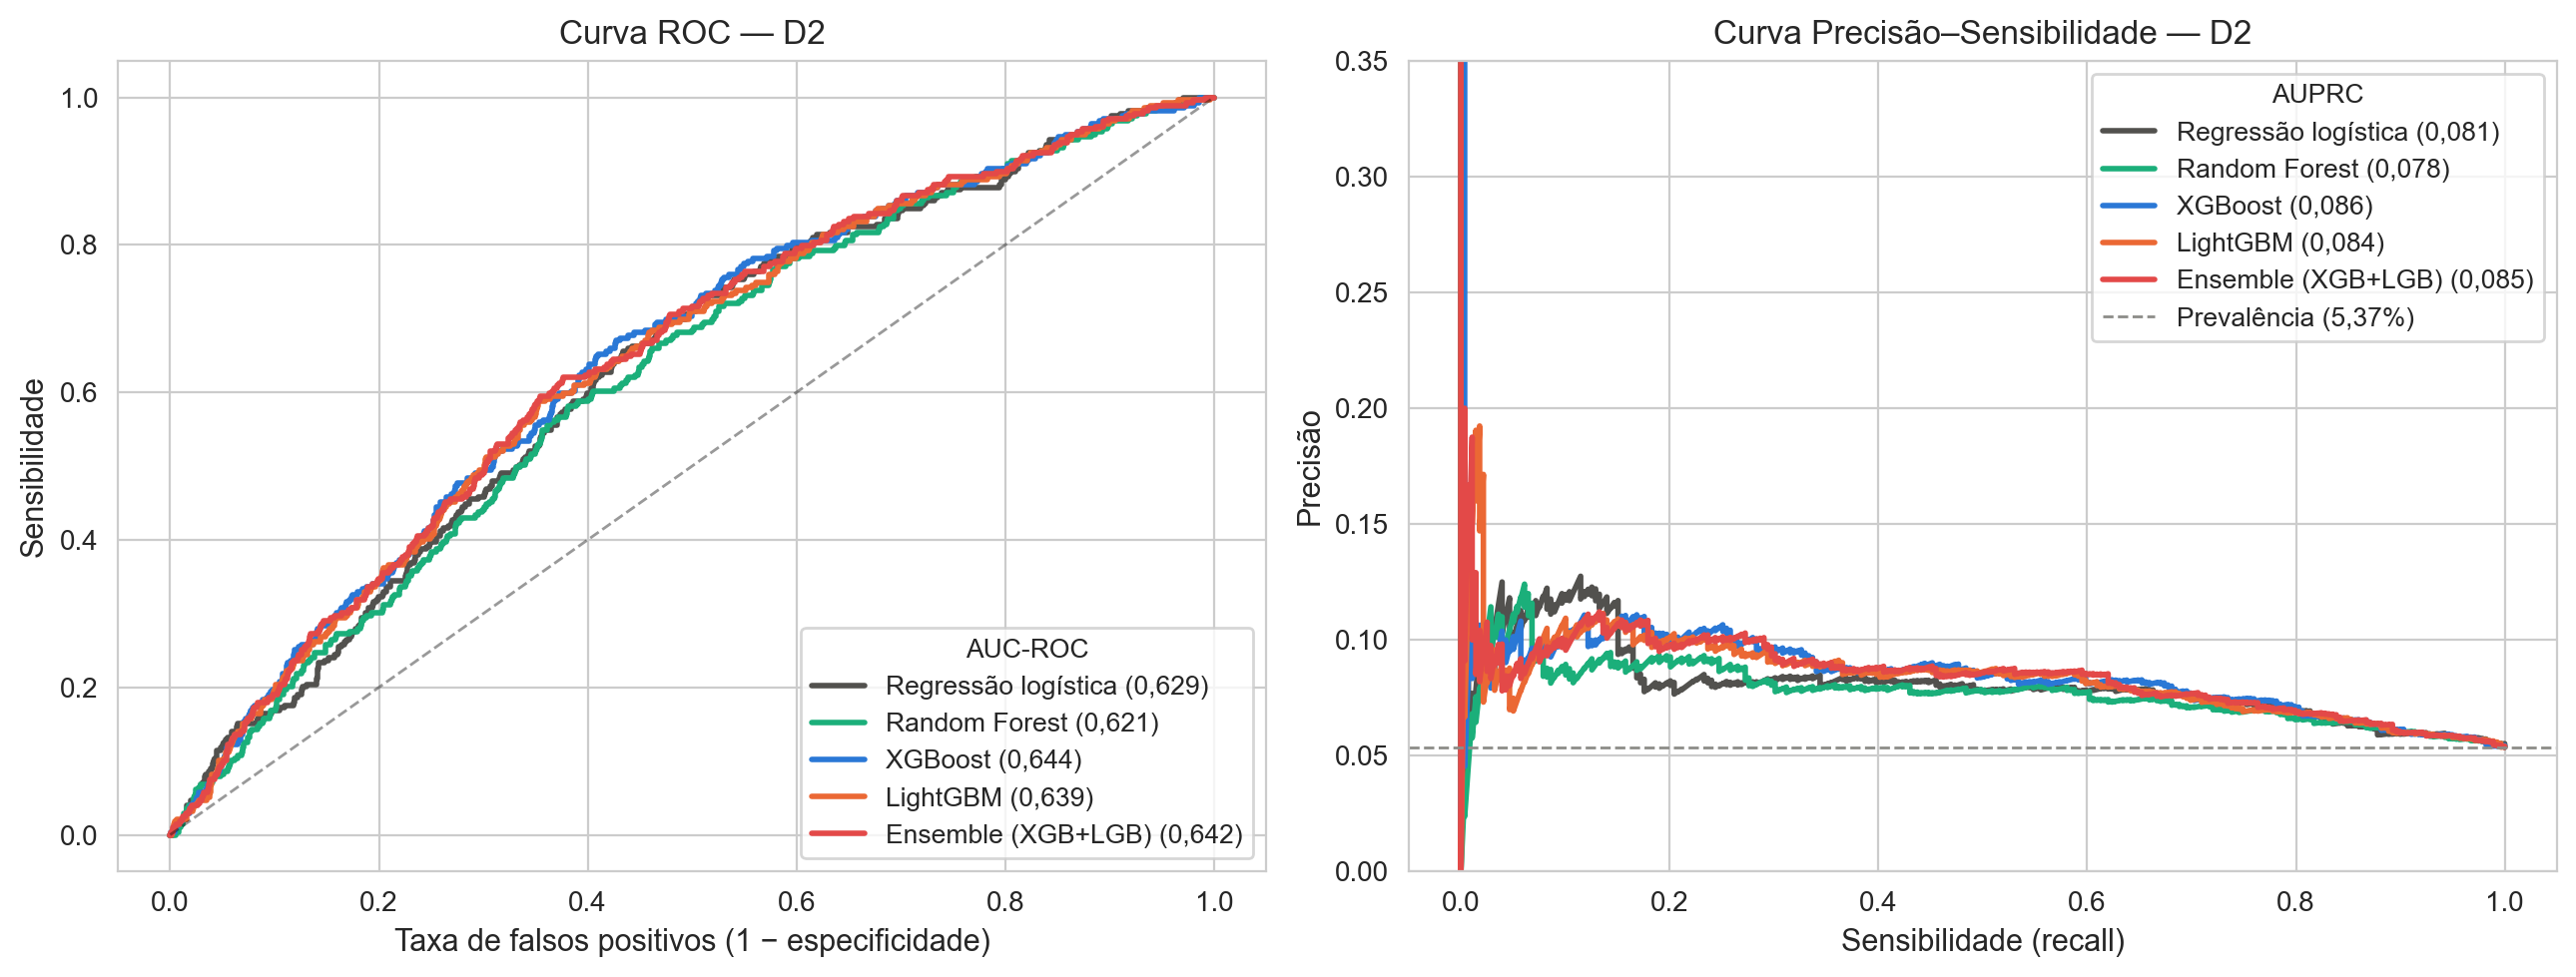
\includegraphics[width=0.92\linewidth]{fig_roc_d2.png}
\caption{Curvas ROC e \textit{Precision--Recall} no corte D2 (conjunto de teste, 5.195 estadias). A linha tracejada na curva PR indica a prevalência do desfecho (5,37\%).}
\label{fig:roc}
\end{figure*}

\begin{table}[!t]
\caption{Métricas completas dos dois melhores modelos}
\label{tab:metricas}
\centering
\small
\begin{tabular}{lcc}
\hline
\textbf{Métrica} & \textbf{XGBoost D2} & \textbf{LightGBM D0} \\
\hline
AUC-ROC              & 0,644 & 0,642 \\
AUPRC                & 0,086 & 0,076 \\
Prevalência no teste & 0,054 & 0,046 \\
\textit{Brier score} & 0,121 & 0,131 \\
Sensibilidade        & 0,624 & 0,613 \\
Precisão             & 0,083 & 0,070 \\
\textit{F1-score}    & 0,146 & 0,125 \\
AUC treino $-$ teste & +0,079 & +0,073 \\
\hline
\end{tabular}
\end{table}

O limiar de decisão foi fixado, em ambos os modelos, no ponto de maior precisão sob a restrição de sensibilidade mínima de 0,60 --- prioriza-se não perder o paciente que retornará. A AUPRC de 0,086 corresponde a 1,60 vezes a prevalência do corte (0,054) --- a referência correta para um desfecho raro, já que a curva ROC é otimista nesse regime \cite{Saito2015}: o ganho sobre o acaso existe, mas é modesto.

\subsection*{C. Evolução Experimental das Configurações}
A Tabela~\ref{tab:evolucao} resume as oito configurações avaliadas, reportando a melhor AUC entre os modelos de cada corte. A progressão é informativa por si só: sete iterações de engenharia de variáveis e otimização de hiperparâmetros moveram o desempenho em D0 de 0,638 para 0,648, e a auditoria final o devolveu a 0,642. O patamar não se move.

\begin{table}[!t]
\caption{Evolução das configurações (melhor AUC por corte)}
\label{tab:evolucao}
\centering
\footnotesize
\begin{tabular}{llcccc}
\hline
\textbf{Ver.} & \textbf{Configuração} & \textbf{D0} & \textbf{D1} & \textbf{D2} & \textbf{D3} \\
\hline
v1 & Divisão aleatória      & 0,638 & 0,673* & 0,634 & 0,627 \\
v2 & Nível de paciente      & 0,642 & 0,630 & 0,634 & 0,613 \\
v3 & + $\Delta$ cumulativo  & 0,642 & 0,633 & 0,630 & 0,613 \\
v4 & + SOFA ponto-no-tempo  & 0,641 & 0,635 & 0,626 & 0,610 \\
v5 & Escores agregados      & 0,619 & 0,621 & 0,604 & 0,586 \\
v6 & + Optuna global        & 0,644 & 0,640 & 0,638 & 0,610 \\
v7 & + Optuna por corte     & 0,648* & 0,646* & 0,644* & 0,610* \\
v8 & $-$ vazamento         & 0,642 & 0,642 & \textbf{0,644} & \textbf{0,619} \\
\hline
\multicolumn{6}{l}{\footnotesize v1: valor inflado pela divisão aleatória, que permitia estadias} \\
\multicolumn{6}{l}{\footnotesize distintas do mesmo paciente em ambos os lados. *v7: inclui o tempo} \\
\multicolumn{6}{l}{\footnotesize total de permanência, removido na v8 (subseção~C).} \\
\end{tabular}
\end{table}

A versão v8 merece explicação separada, por ser a única que \textit{reduz} o desempenho deliberadamente. A auditoria do conjunto de variáveis descrita na subseção~III-C removeu o tempo total de permanência na UTI, a binária dela derivada e a unidade de alta redundante. O efeito, medido com os hiperparâmetros da v7 fixos no corte D0, foi de $-$0,002 em AUC para o XGBoost. Após reotimização completa, o resultado se redistribui entre os cortes: D0 e D1 perdem cerca de 0,005, enquanto D3 \textit{ganha} entre 0,003 e 0,011 --- a variável removida vinha prejudicando justamente o corte em que sua faixa de valores é mais truncada. O modelo final passa a ser o XGBoost em D2, e o sobreajuste do melhor modelo cai de +0,146 para +0,079. Paga-se 0,004 de AUC no valor de destaque em troca de um modelo que só usa informação disponível no instante da predição e que generaliza melhor.

Três resultados negativos merecem registro. Primeiro, a v1 ilustra o efeito do vazamento, cuja tipologia e prevalência na literatura estão catalogadas \cite{Kapoor2023}: a AUC aparentemente superior em D1 (0,673) desapareceu ao se adotar a divisão em nível de paciente, caindo para 0,630. Segundo, os deltas calculados entre \textit{snapshots} cumulativos (v3) não produziram efeito algum --- como os \textit{snapshots} agregam por máximo ou mínimo desde a admissão, a diferença entre dois cortes consecutivos é sempre não negativa para agregações de máximo, de modo que o modelo nunca observa recuperação clínica. A correção adotada na v4 foi calcular a trajetória sobre janelas móveis de 24 horas, e não sobre janelas cumulativas. Terceiro, substituir as variáveis fisiológicas brutas pelos escores de gravidade consolidados (v5) degradou o desempenho em todos os cortes: a agregação em escore descarta informação que o modelo aproveita.

\subsection*{D. \textit{Snapshots} Independentes \textit{versus} Modelo de Trajetória}
Para testar se a trajetória completa carrega sinal além do último corte, treinou-se um modelo com D0, D1, D2 e D3 concatenados (421 variáveis), comparado contra o D3 restrito à mesma coorte de pacientes com permanência de ao menos 96 horas.

\begin{table}[!t]
\caption{Modelo de trajetória D0$\rightarrow$D3 \textit{versus} D3 isolado (mesma coorte)}
\label{tab:trajetoria}
\centering
\small
\begin{tabular}{lccc}
\hline
\textbf{Modelo} & \textbf{D3 (LOS $\geq$ 96 h)} & \textbf{D0$\rightarrow$D3} & \textbf{$\Delta$} \\
\hline
Regressão logística & 0,610 & 0,582 & $-$0,028 \\
Random Forest       & 0,611 & 0,602 & $-$0,009 \\
XGBoost             & 0,616 & 0,606 & $-$0,010 \\
LightGBM            & 0,615 & 0,597 & $-$0,018 \\
Ensemble            & 0,616 & 0,603 & $-$0,013 \\
\hline
\end{tabular}
\end{table}

O corte isolado supera a trajetória concatenada em todos os modelos. Com 14.444 amostras de treino e cerca de 800 eventos positivos, 421 variáveis constituem dimensionalidade excessiva. O resultado sustenta a arquitetura adotada: \textit{snapshots} cumulativos com variáveis de trajetória em janela móvel já codificam a evolução do paciente de forma mais eficiente que a concatenação explícita dos cortes anteriores.

\subsection*{E. Explicabilidade do Modelo Final}
A interpretação foi obtida por TreeSHAP \cite{Lundberg2017,Lundberg2020} aplicado ao modelo final sobre o conjunto de teste --- a exigência de explicabilidade é apontada como condição para a adoção clínica de modelos preditivos \cite{Kelly2019}. Para garantir a auditabilidade, o procedimento reconstrói o conjunto de teste a partir do modelo serializado e recalcula a AUC antes de computar as atribuições, confirmando que as figuras derivam exatamente do modelo que produziu as métricas reportadas.

\begin{figure*}[!t]
\centering
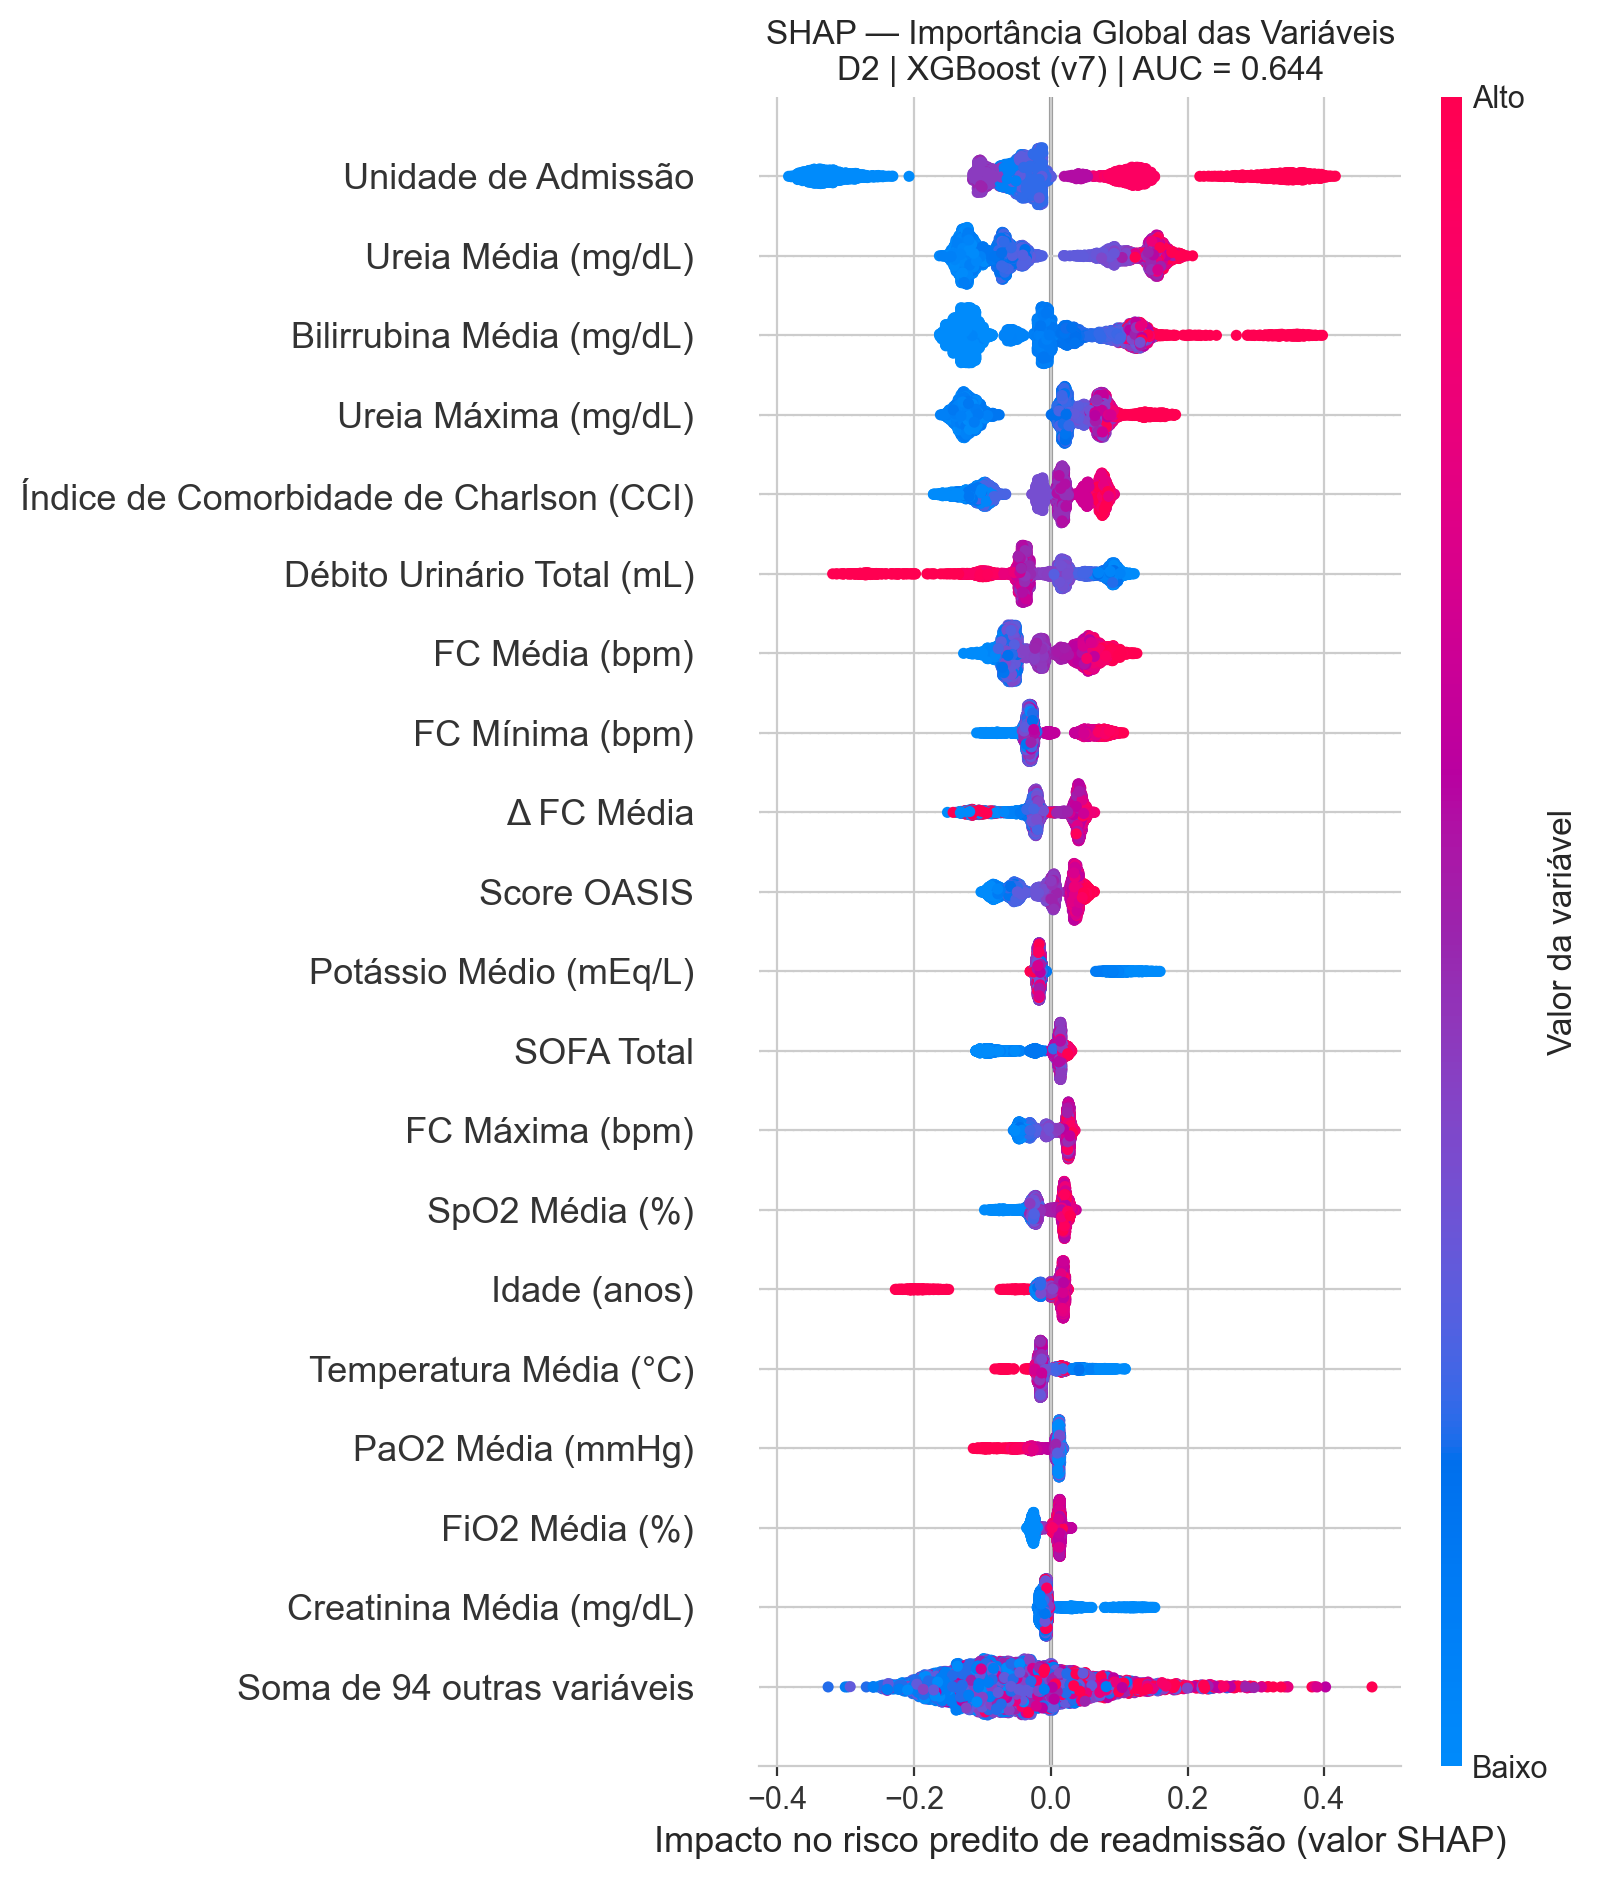
\includegraphics[width=0.66\linewidth]{fig_shap_beeswarm_d2.png}
\caption{Contribuição das 20 variáveis mais influentes no corte D2 (XGBoost, modelo final). Cada ponto é uma estadia; a posição horizontal indica o impacto no risco predito e a cor, o valor da variável.}
\label{fig:shap}
\end{figure*}

A leitura mais informativa não vem de um corte isolado, mas da comparação entre eles. Aplicando o mesmo algoritmo aos três primeiros cortes, obtém-se a evolução da importância relativa ao longo da internação (Tabela~\ref{tab:shaptempo}).

\begin{table}[!t]
\caption{Posição e impacto médio (\(|\)SHAP\(|\)) das principais variáveis, por corte temporal (XGBoost)}
\label{tab:shaptempo}
\centering
\small
\begin{tabular}{lccc}
\hline
\textbf{Variável} & \textbf{D0} & \textbf{D1} & \textbf{D2} \\
\hline
Comorbidade (Charlson) & 1º / 0,175 & 3º / 0,108 & 5º / 0,060 \\
Unidade de admissão    & 2º / 0,129 & 1º / 0,128 & 1º / 0,140 \\
Ureia média            & 3º / 0,101 & 2º / 0,121 & 2º / 0,110 \\
Bilirrubina média      & 9º / 0,044 & 5º / 0,066 & 3º / 0,093 \\
Débito urinário        & 5º / 0,066 & 7º / 0,057 & 6º / 0,056 \\
SOFA em janela móvel   & 21º / 0,013 & 6º / 0,058 & 20º / 0,015 \\
\hline
\end{tabular}
\end{table}

Quatro leituras emergem. A primeira, e a mais relevante para a arquitetura proposta, é que \textbf{a carga crônica de doença perde peso à medida que a observação fisiológica se acumula}: o índice de comorbidade de Charlson \cite{Charlson1987} é a variável mais influente em D0, cai para terceira em D1 e para quinta em D2, com o impacto médio reduzido a um terço. Nas primeiras 24 horas o modelo dispõe de pouco mais que o perfil basal do paciente; a partir de 72 horas, o estado agudo passa a carregar o sinal. Um classificador único, treinado sobre um recorte fixo, não exporia esse deslocamento.

A segunda é a consistência do eixo renal, o sinal mais estável do modelo: a ureia média ocupa a segunda ou terceira posição nos três cortes e o débito urinário permanece entre a quinta e a sétima, com direção fisiologicamente correta --- ureia elevada e diurese reduzida aumentam o risco, em concordância com os critérios que definem disfunção renal aguda \cite{KDIGO2012}.

A terceira é o percurso inverso da disfunção hepática: a bilirrubina média sobe de nona para terceira posição entre D0 e D2. Comorbidade e disfunção orgânica adquirida trocam de papel ao longo da internação.

A quarta é que os escores consolidados não dominam. O OASIS \cite{JohnsonOASIS2013} não passa da sexta posição em nenhum corte, e o SOFA \cite{Vincent1996} em janela móvel é marginal em D0, atinge a sexta posição em D1 --- quando 48 horas de observação tornam a gravidade pontual informativa --- e volta a cair em D2, momento em que as variáveis laboratoriais acumuladas já carregam a mesma informação. O resultado converge com o negativo da v5: agregar em escore descarta sinal que o modelo aproveita nas variáveis brutas. As 31 variáveis de trajetória, por sua vez, respondem por 13,3\% do \(|\)SHAP\(|\) somado em D1 e 11,4\% em D2 --- contribuem, mas não dominam.

A unidade de internação merece tratamento à parte. Trata-se de variável nominal codificada por rótulos, de modo que qualquer leitura monotônica sobre o código seria artefato da ordenação alfabética. A forma interpretável é por categoria (Fig.~\ref{fig:unidades}): a correlação entre a contribuição média por unidade e a taxa de readmissão efetivamente observada em cada uma é de 0,71, evidenciando que o modelo aprendeu risco real de unidade --- a unidade de trauma cirúrgico concentra a maior contribuição positiva e a maior taxa observada (9,5\%), ao passo que as unidades neurológicas intermediárias ficam no extremo oposto. Cabe a ressalva de que a atribuição SHAP é condicional: unidades como a coronariana e a clínica apresentam taxa observada próxima à da unidade cirúrgica, mas contribuição negativa, porque nelas o risco já é explicado por outras variáveis do próprio paciente.

\begin{figure}[!t]
\centering
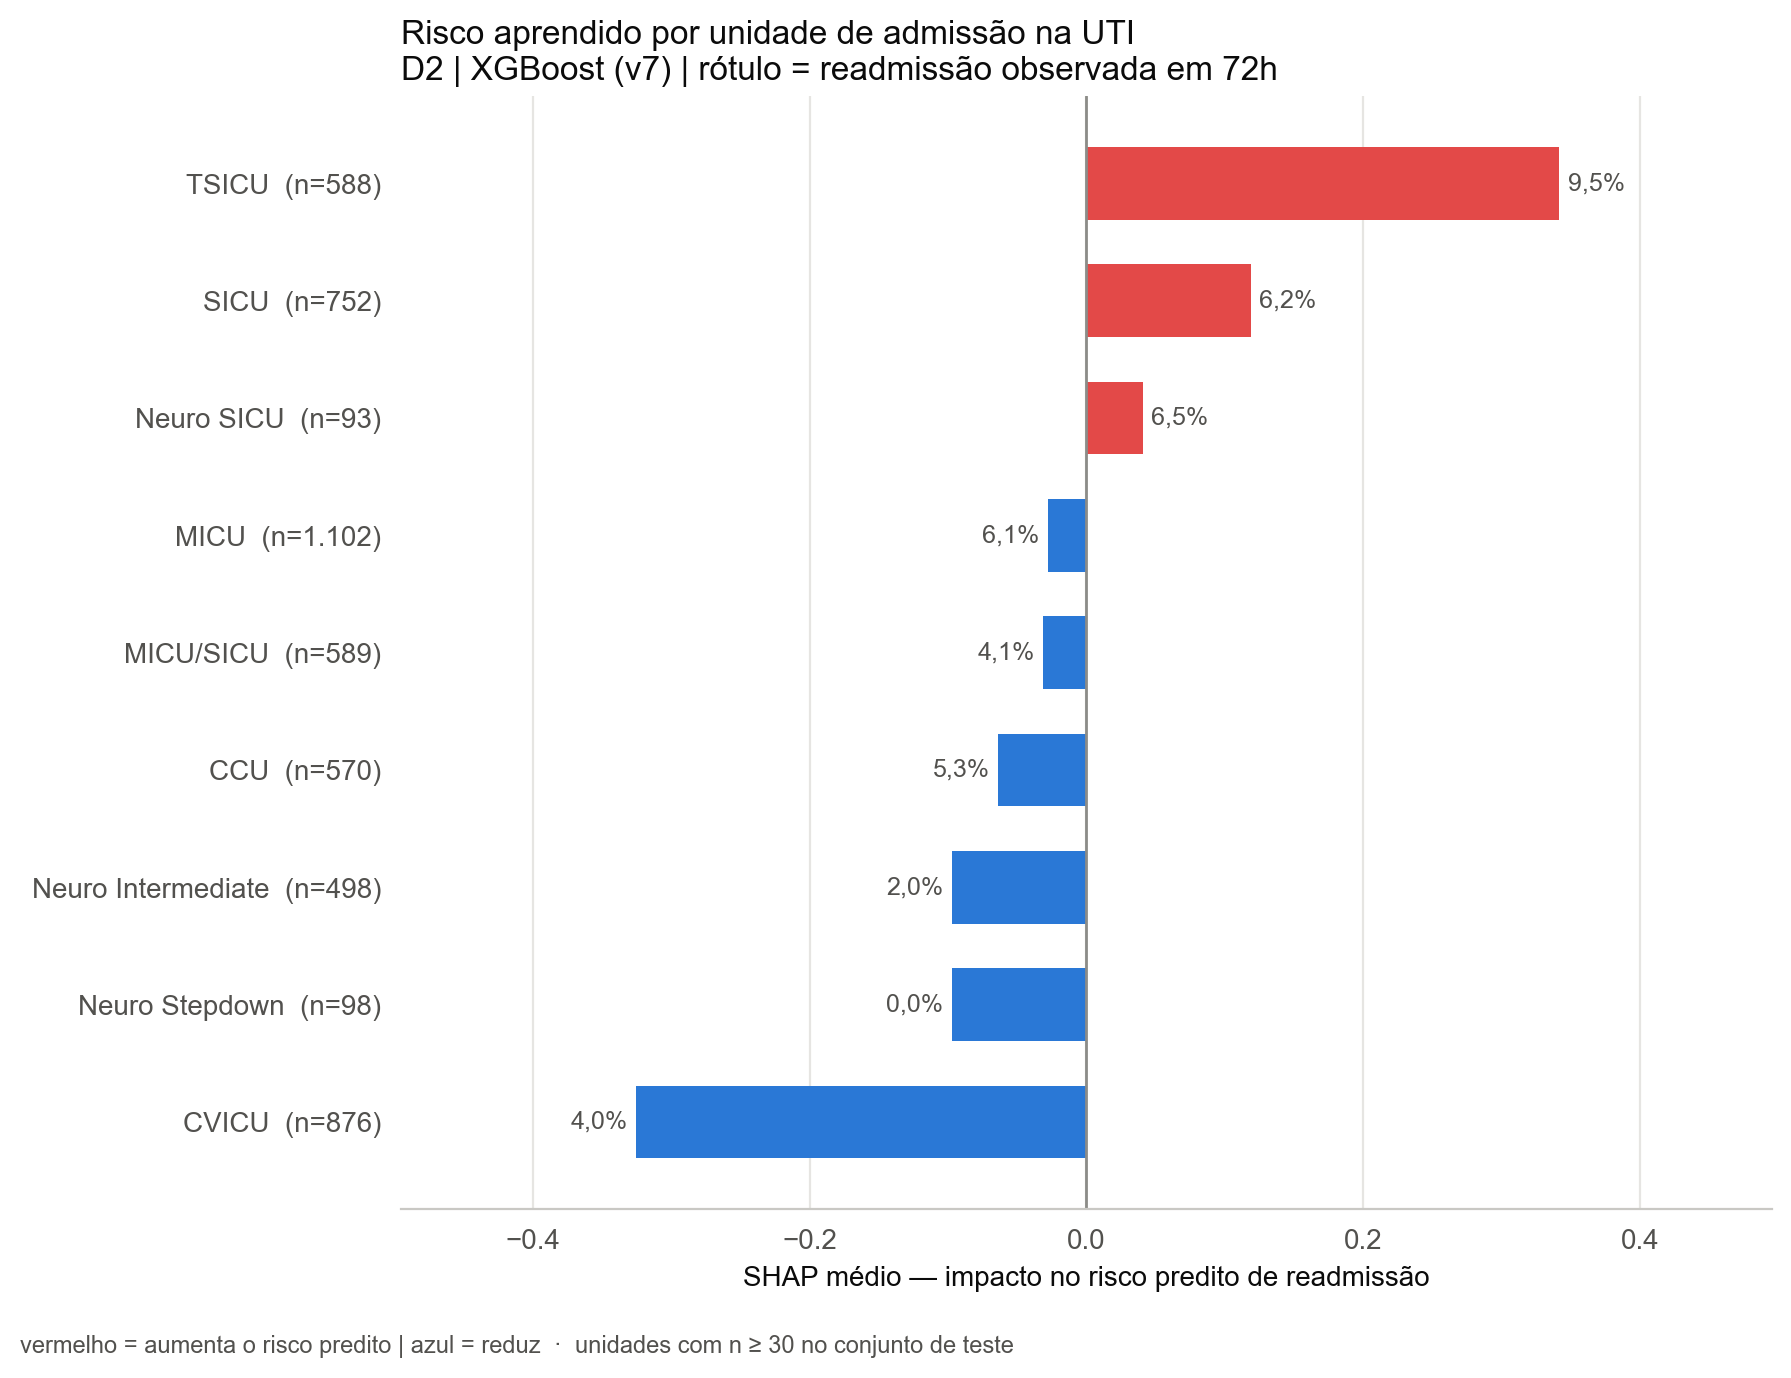
\includegraphics[width=\linewidth]{fig_shap_unidades_d2.png}
\caption{Contribuição média por unidade de internação (D2, XGBoost). O rótulo de cada barra indica a taxa de readmissão observada na unidade.}
\label{fig:unidades}
\end{figure}

\subsection*{F. Métrica Operacional e Calibração}
A previsão agregada --- somar as probabilidades individuais para estimar quantos pacientes retornarão em uma janela --- é o elemento operacional da arquitetura de referência \cite{King2022}. Sua aplicação direta aos modelos aqui obtidos, entretanto, não é válida: no corte D2, a soma das probabilidades preditas no conjunto de teste estima 1.601 readmissões contra 279 observadas, uma superestimação de 474\%. O \textit{Brier score} confirma o diagnóstico: 0,121 contra 0,051 de um preditor constante igual à prevalência. A dissociação entre boa discriminação e calibração ruim é um modo de falha conhecido e frequentemente não reportado \cite{VanCalster2019}.

A causa é conhecida e é consequência direta de uma escolha de projeto. O uso de \texttt{scale\_pos\_weight} para compensar o desbalanceamento otimiza a \textit{ordenação} de risco às custas do \textit{nível absoluto} das probabilidades. O modelo é útil para priorizar pacientes --- que é o uso clínico pretendido ---, mas suas saídas não são probabilidades calibradas e não podem ser somadas. A obtenção da métrica operacional exige uma etapa adicional de recalibração (por regressão logística de Platt ou regressão isotônica), ajustada em um conjunto de validação separado \cite{VanCalster2019}, registrada aqui como trabalho futuro. Reporta-se o achado explicitamente porque a combinação de ponderação de classes com métricas de calibração é frequente na literatura de readmissão e raramente discutida.

No ponto de operação escolhido, o modelo sinaliza 2.101 das 5.195 estadias de teste (40,4\%) para capturar 62\% dos eventos, com precisão de 0,083 --- ou seja, aproximadamente 12 pacientes sinalizados para cada readmissão efetivamente identificada, contra 19 esperados pelo acaso. É um ganho real, porém insuficiente para acionar intervenções de alto custo, e adequado apenas a intervenções de baixo custo, como a revisão estruturada da decisão de alta.

\subsection*{G. Desempenho Frente à Literatura}
A proposta inicial deste trabalho registrava a expectativa de AUROC superior a 0,80 como indicativo de viabilidade clínica. Essa expectativa não se sustenta diante da literatura recente quando o desenho experimental é levado em conta, e sua revisão é, em si, um resultado.

A revisão sistemática mais abrangente sobre o tema \cite{Koumantakis2025} reuniu 24 estudos e 49 modelos de aprendizado profundo para readmissão em UTI. A AUROC agregada dos 11 estudos passíveis de meta-análise foi de 0,79 (IC 95\% 0,73--0,85), com $I^2 = 99{,}96\%$ --- heterogeneidade praticamente total, o que significa que os desempenhos publicados não são comparáveis entre si. Apenas dois dos 24 estudos realizaram validação externa e, em um deles, a AUROC caiu de 0,80 para 0,55 fora da base de origem.

A mesma revisão oferece o fator que explica boa parte da dispersão: modelos restritos a subpopulações de uma doença específica alcançam AUROC média de 0,92 (IC 95\% 0,89--0,95) com heterogeneidade baixa ($I^2 = 17{,}1\%$; $p = 0{,}002$), muito acima dos modelos de UTI geral. O estudo mais citado em readmissão de UTI com MIMIC \cite{Miao2024} é exatamente desse tipo: restringe-se a 2.242 pacientes com hemorragia intracerebral, população cuja taxa de readmissão (9,6\% no MIMIC-III e 10,6\% no MIMIC-IV) é aproximadamente o dobro da observada na coorte geral deste trabalho (4,5\%), e reporta AUC de 0,736 (IC 95\% 0,668--0,801). Comparar esse valor diretamente com o obtido aqui é comparar populações distintas.

Há ainda o efeito do tratamento do desbalanceamento. O trabalho citado emprega SMOTEENN, e demonstrou-se que aplicar reamostragem sintética antes da validação cruzada produz viés de até 0,34 em AUC \cite{Demircioglu2024}, porque amostras sintéticas derivadas do conjunto de teste vazam para o treino. O problema não é isolado: um levantamento sistemático identificou vazamento de dados afetando ao menos 294 artigos em 17 disciplinas \cite{Kapoor2023}.

Por fim, há uma referência positiva de rigor metodológico. O modelo iREAD \cite{Lim2025}, desenvolvido em coorte de 70.842 pacientes com divisão temporal e validação externa multicêntrica, obteve AUROC de 0,820 na validação interna, 0,768 no MIMIC-III e 0,725 no eICU-CRD. Mesmo um modelo construído com rigor perde cerca de 0,10 de AUROC ao sair do hospital de origem.

O valor de 0,644 obtido neste trabalho --- com divisão em nível de paciente, sem reamostragem sintética, sem imputação de variáveis ausentes, com auditoria explícita do conjunto de variáveis quanto a informação indisponível no instante da predição, e em população de UTI geral --- deve ser lido como uma linha de base honesta para o problema, e não como desempenho inferior. A conclusão prática é que o critério de viabilidade clínica não pode ser um limiar de AUROC: precisa ser o ponto de operação, o custo da intervenção associada e o desempenho sob validação externa.

\subsection*{H. Simulação de Uso Clínico}
Como prova de conceito da camada de entrega, foi implementada uma interface em Streamlit que carrega os modelos serializados dos quatro cortes e opera em dois modos: consulta por identificador de estadia, recuperando os \textit{snapshots} disponíveis do paciente, e carregamento de um arquivo CSV com os dados de um paciente novo. Para cada corte disponível a interface apresenta a probabilidade de readmissão, a evolução do risco ao longo dos cortes e a decomposição SHAP individual (Fig.~\ref{fig:waterfall}), que mostra quais variáveis elevaram e quais reduziram o risco daquele paciente específico em relação à média da coorte.

\begin{figure}[!t]
\centering
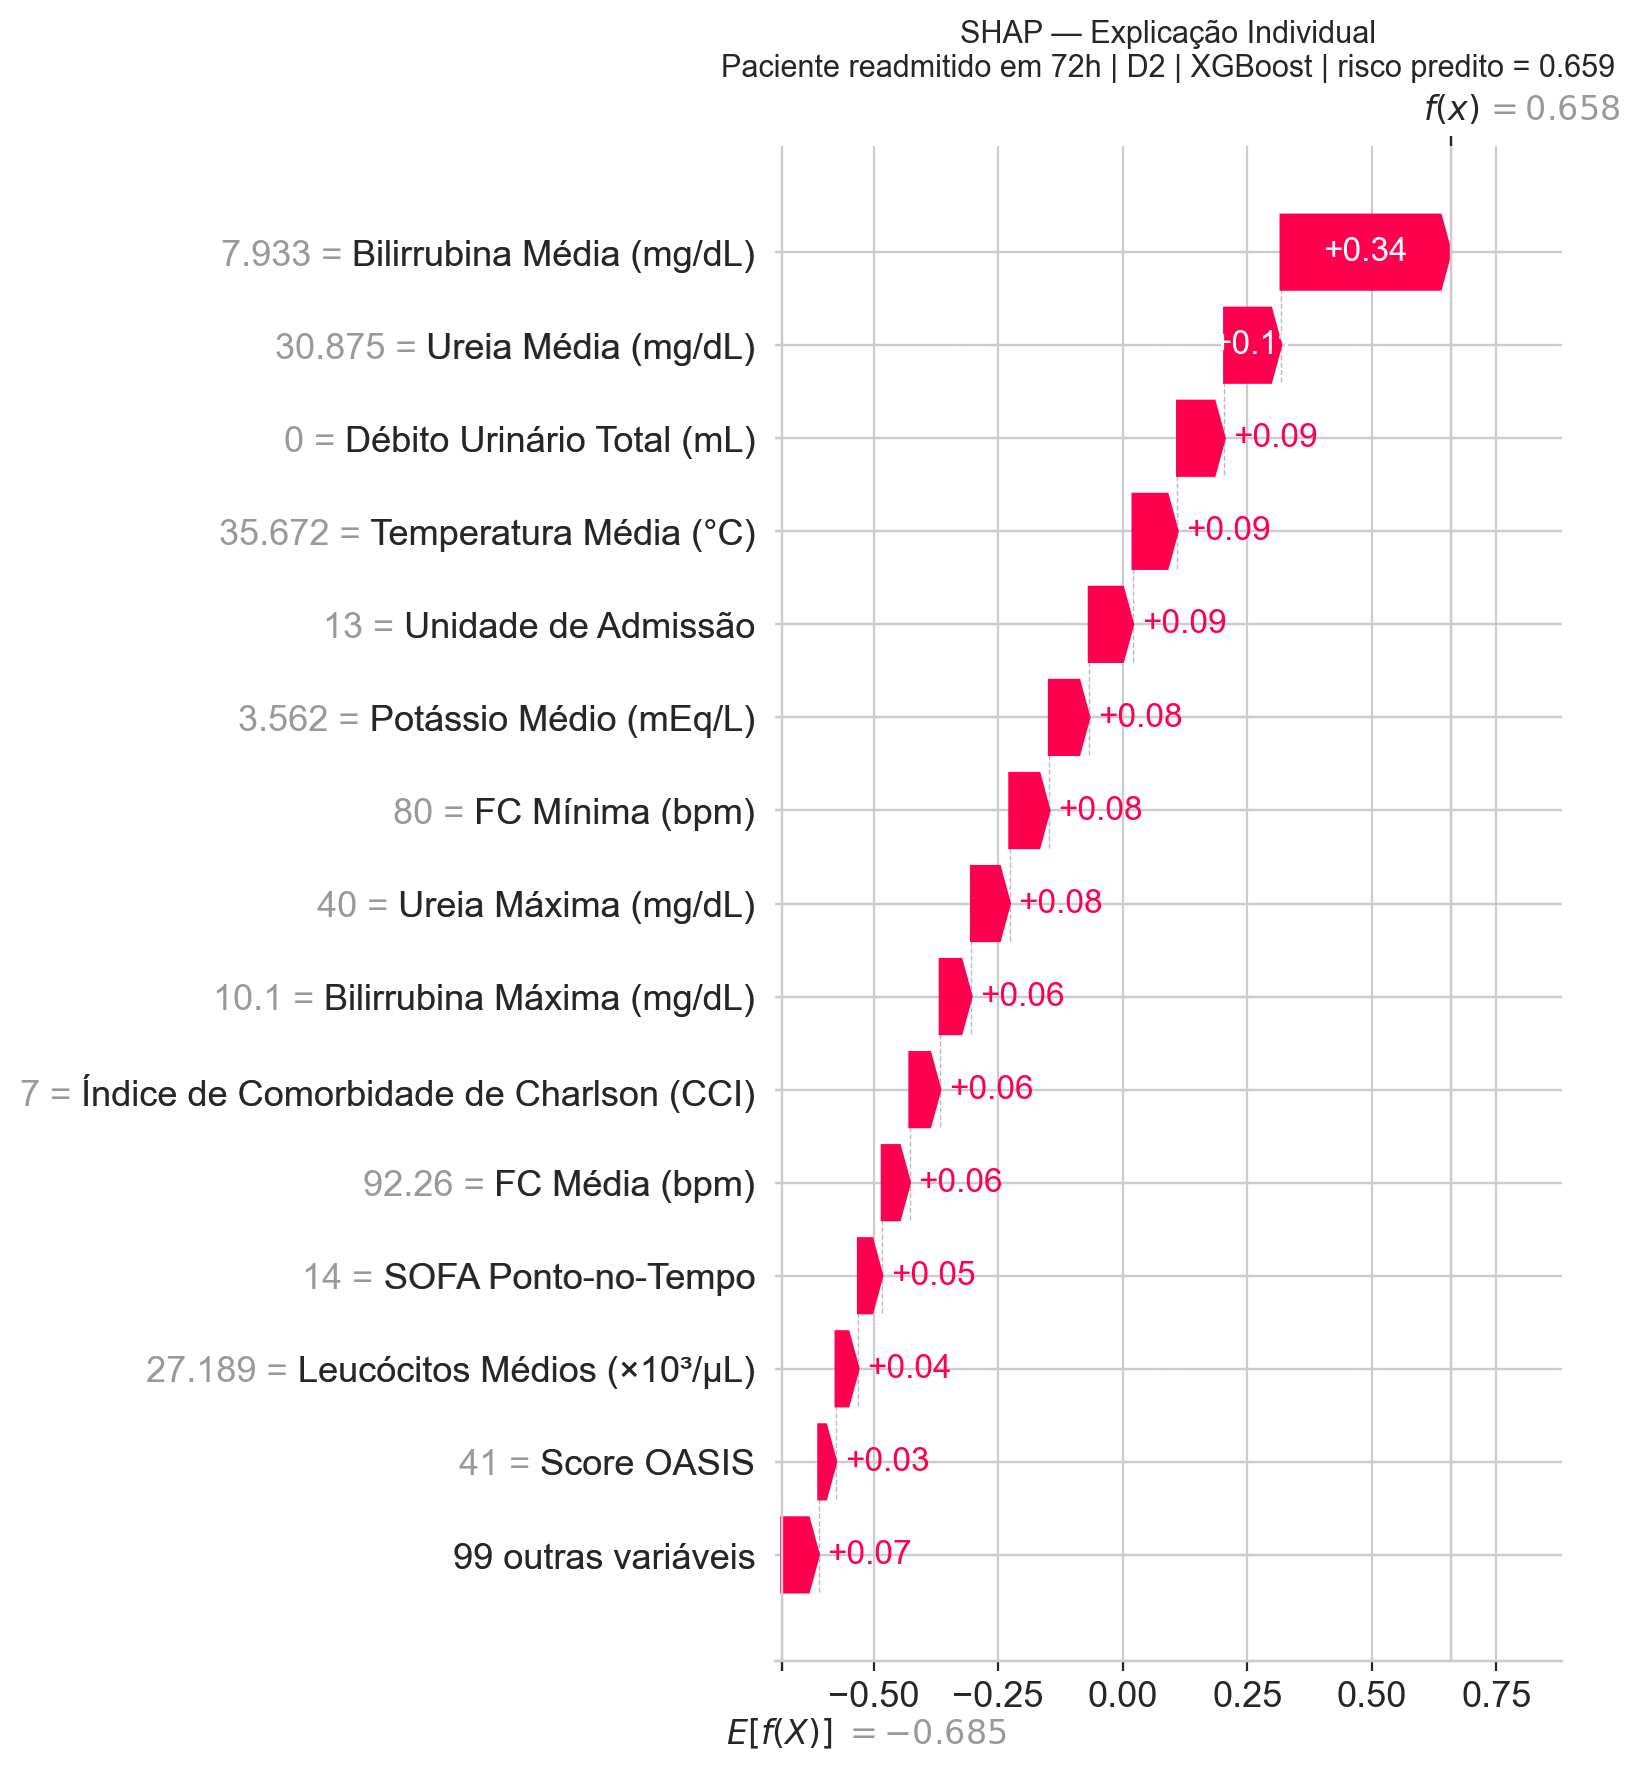
\includegraphics[width=\linewidth]{fig_shap_waterfall_d2.png}
\caption{Decomposição SHAP individual de um paciente readmitido em 72 horas (corte D2, risco predito 0,659). As barras indicam a contribuição de cada variável em relação ao valor esperado do modelo.}
\label{fig:waterfall}
\end{figure}

A decomposição individual é o que torna a predição acionável \cite{Lundberg2020}: um risco de 0,66 sem justificativa é uma caixa-preta, ao passo que a indicação de que bilirrubina média de 7,9 mg/dL, ureia de 30,9 mg/dL, anúria no período e hipotermia de 35,7 \textcelsius{} foram os principais responsáveis pelo valor permite ao clínico avaliar se o alerta é plausível --- e, neste caso, o conjunto descreve um quadro de disfunção orgânica múltipla que justifica o alerta.

\subsection*{I. Limitações e Trabalhos Futuros}
A principal limitação é o teto de desempenho: com dados exclusivamente intra-UTI, o patamar de 0,65 mostrou-se estável frente a sete configurações distintas de \textit{features} e hiperparâmetros. Parte do sinal relevante para a readmissão provavelmente está fora do escopo destes dados --- condições da enfermaria de destino, disponibilidade de leitos, horário da alta, suporte familiar e adesão a protocolos de alta, fatores que a literatura de readmissão precoce associa ao desfecho \cite{Badilla2025}.

As demais limitações são: ausência de validação externa, o que impede afirmar generalização --- e a literatura mostra que a perda nessa transição é substancial \cite{Koumantakis2025,Lim2025} e que o deslocamento de distribuição entre instituições é a regra, não a exceção \cite{Finlayson2021}; ausência de calibração, discutida na subseção~F, que impede o uso agregado das probabilidades; o viés de seleção entre cortes, que torna D0 e D3 populações distintas; e o \textit{overfitting} residual de +0,079 entre treino e teste no modelo final, apesar da regularização ajustada por Optuna.

Como trabalhos futuros, destacam-se a recalibração das probabilidades e a consequente obtenção da métrica operacional agregada; a validação externa em base independente, preferencialmente o eICU-CRD \cite{Pollard2018}, cuja natureza multicêntrica submeteria o modelo à variação entre instituições; a incorporação de dados pós-alta da enfermaria, que testaria diretamente a hipótese sobre a origem do teto de desempenho; e a avaliação de estratégias de mitigação de \textit{concept drift} em operação contínua.

Ressalta-se, ainda, que a base MIMIC-IV é oriunda de hospitais dos Estados Unidos \cite{Johnson2023}, cujos protocolos clínicos, infraestrutura e perfil populacional podem diferir significativamente da realidade brasileira --- uma forma de deslocamento de distribuição cujo efeito sobre o desempenho é bem documentado \cite{Finlayson2021}. Dessa forma, embora útil para validação inicial do modelo, recomenda-se que o treinamento final seja realizado com bases de dados nacionais ou diretamente com os dados do hospital de destino, garantindo maior aderência ao contexto local e melhor desempenho na prática clínica.


% ---------------------------------------------------------
% 5. Conclusão
% ---------------------------------------------------------
\section{Conclusão}
Este trabalho apresenta uma arquitetura modular de ML para previsão de readmissão em UTI baseada na MIMIC-IV. A adoção de \textit{snapshots} temporais, recalibração contínua e métricas operacionais aproxima a pesquisa de um cenário real, oferecendo um caminho pragmático para transpor modelos acadêmicos à prática clínica. A abordagem pode ser generalizada para outros eventos (mortalidade, tempo de permanência) e outros contextos hospitalares, desde que respeitados os princípios de MLOps \cite{Kreuzberger2023}, a validação externa \cite{Koumantakis2025} e a governança de dados clínicos \cite{Bender2013}.

% ---------------------------------------------------------
% Agradecimentos (opcional)
% ---------------------------------------------------------
\section*{Agradecimentos}
Agradeço especialmente aos professores do IFSC pelo apoio, orientação e pela oportunidade de explorar um tema tão complexo e emergente como a aplicação de aprendizado de máquina na área da saúde. Também agradeço à comunidade MIMIC, aos revisores anônimos e aos colegas que contribuíram com discussões sobre arquitetura de dados hospitalares e MLOps.

% ---------------------------------------------------------
% Referências
% ---------------------------------------------------------
\bibliography{mylibrary}
\bibliographystyle{IEEEtran}

\EOD

\end{document}

